\documentclass[11pt]{article}

\usepackage{latexsym}
\usepackage{amsmath}
\usepackage{amssymb}
\usepackage{amsthm}
\usepackage{graphicx}
\usepackage{wrapfig}
\usepackage{pseudocode}
\usepackage{url}
\usepackage[backref, colorlinks=true, citecolor=red, urlcolor=blue, pdfauthor={Jyh-Ming Lien}]{hyperref}


\newcommand{\handout}[5]{
  \noindent
  \begin{center}
  \framebox{
    \vbox{
      \hbox to 5.78in { {\bf } \hfill #2 }
      \vspace{4mm}
      \hbox to 5.78in { {\Large \hfill #5  \hfill} }
      \vspace{2mm}
      \hbox to 5.78in { {\em #3 \hfill #4} }
    }
  }
  \end{center}
  \vspace*{4mm}
}

\newcommand{\lecture}[4]{\handout{#1}{#2}{#3}{#4}{#1}}

\newtheorem{theorem}{Theorem}
\newtheorem{corollary}[theorem]{Corollary}
\newtheorem{lemma}[theorem]{Lemma}
\newtheorem{observation}[theorem]{Observation}
\newtheorem{proposition}[theorem]{Proposition}
\newtheorem{definition}[theorem]{Definition}
\newtheorem{claim}[theorem]{Claim}
\newtheorem{fact}[theorem]{Fact}
\newtheorem{assumption}[theorem]{Assumption}

% 1-inch margins, from fullpage.sty by H.Partl, Version 2, Dec. 15, 1988.
\topmargin 0pt
\advance \topmargin by -\headheight
\advance \topmargin by -\headsep
\textheight 8.9in
\oddsidemargin 0pt
\evensidemargin \oddsidemargin
\marginparwidth 0.5in
\textwidth 6.5in

\parindent 0in
\parskip 1.5ex
%\renewcommand{\baselinestretch}{1.25}

\begin{document}

\lecture{Assignment3 Report}{Fall 2017}{Genqian Hu}{Computational Geometry}

\section{Summary of the two methods}

\subsection{hedcuter method}
\subsubsection{Voronoi diagram and Centroidal Voronoi tessellation}
\paragraph{First, the algorithm resizes the input image to a larger virtual image. Then, it scans the cells and stores all sites in a heap. After, it pops a cell to compute dx and dy so to get the centroidal voronoi diagram. When all cells are visited and the heap is empty, it collects cells from (0,0) rightwards and then remove empty cells. Finally, it moves each cell to its center of its coverage.}
\subsubsection{stippling}
\paragraph{It reads the image and the centroidal voronoi tessellation computed before to stipple. It retrieves each cell from CVT and its grayscale information. Then, the location of each disk is defined by the x and y coordinates of each sites of the cells retrieved. The color of it is determinded by grayscale value. If it is required a colorful output, then the rgb value is from the original image's rgb value at that pixel.}
\subsection{voronoi method}
\paragraph{First, it computes the range of the coordinates of the sites. Then do the plane sweep, if the sites' y coordinate is bigger than the lowest intersection's, it determines which half edge the new site intersects with and will triangulate it. If the sites' y is smaller, it creates a new bisector between the left and right half edges. Finally, it scans the edges and eliminates the invalid edges. }
\subsubsection{Centroidal Voronoi tessellation}
\paragraph{It adds clip lines to the voronoi digrams one by one. If the density is higher there, the x and y there will also get larger weight when computing the new centroid. If no points are outside the clip planes,the centroid is computed by the sum of coordinates and the density there. }
\subsubsection{stippling}
\paragraph{It read the coordinates of all the centroids created before. Then it outputs them to the output file. And it assigns each of them the right color as needed.}
\section{Comparison of the two methods}
\begin{figure}[h!]
\centering
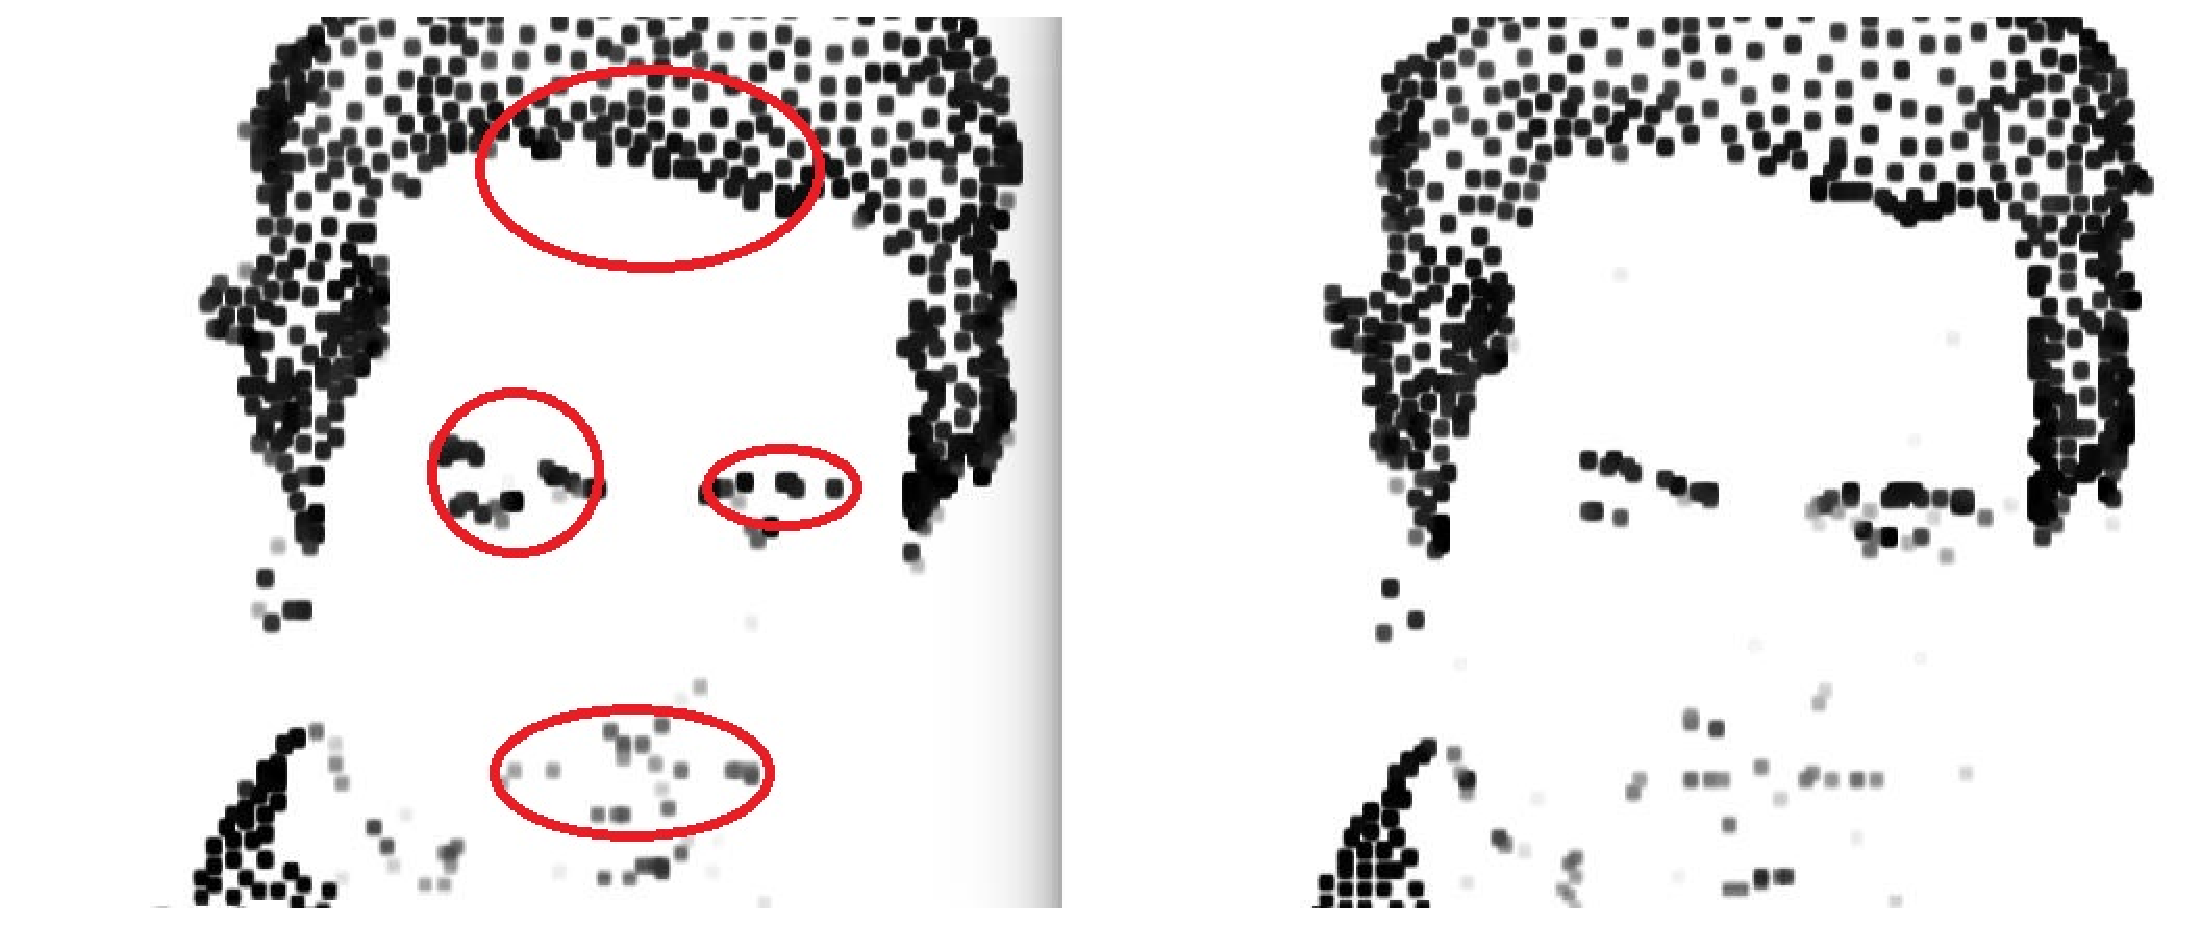
\includegraphics[width=0.80\textwidth]{figure1.eps}
\caption{Different outputs from hedcuter}
\label{threadsVsSync}
\end{figure}
\paragraph{1. The output images from hedcuter are different as shown in Figure 1. But the output images from voronoi are the same. Because hedcuter uses rng\_uniorm and rng\_gaussian methods to randomly initial points, the details is normal to be different during each run.}

\begin{figure}[h!]
\centering
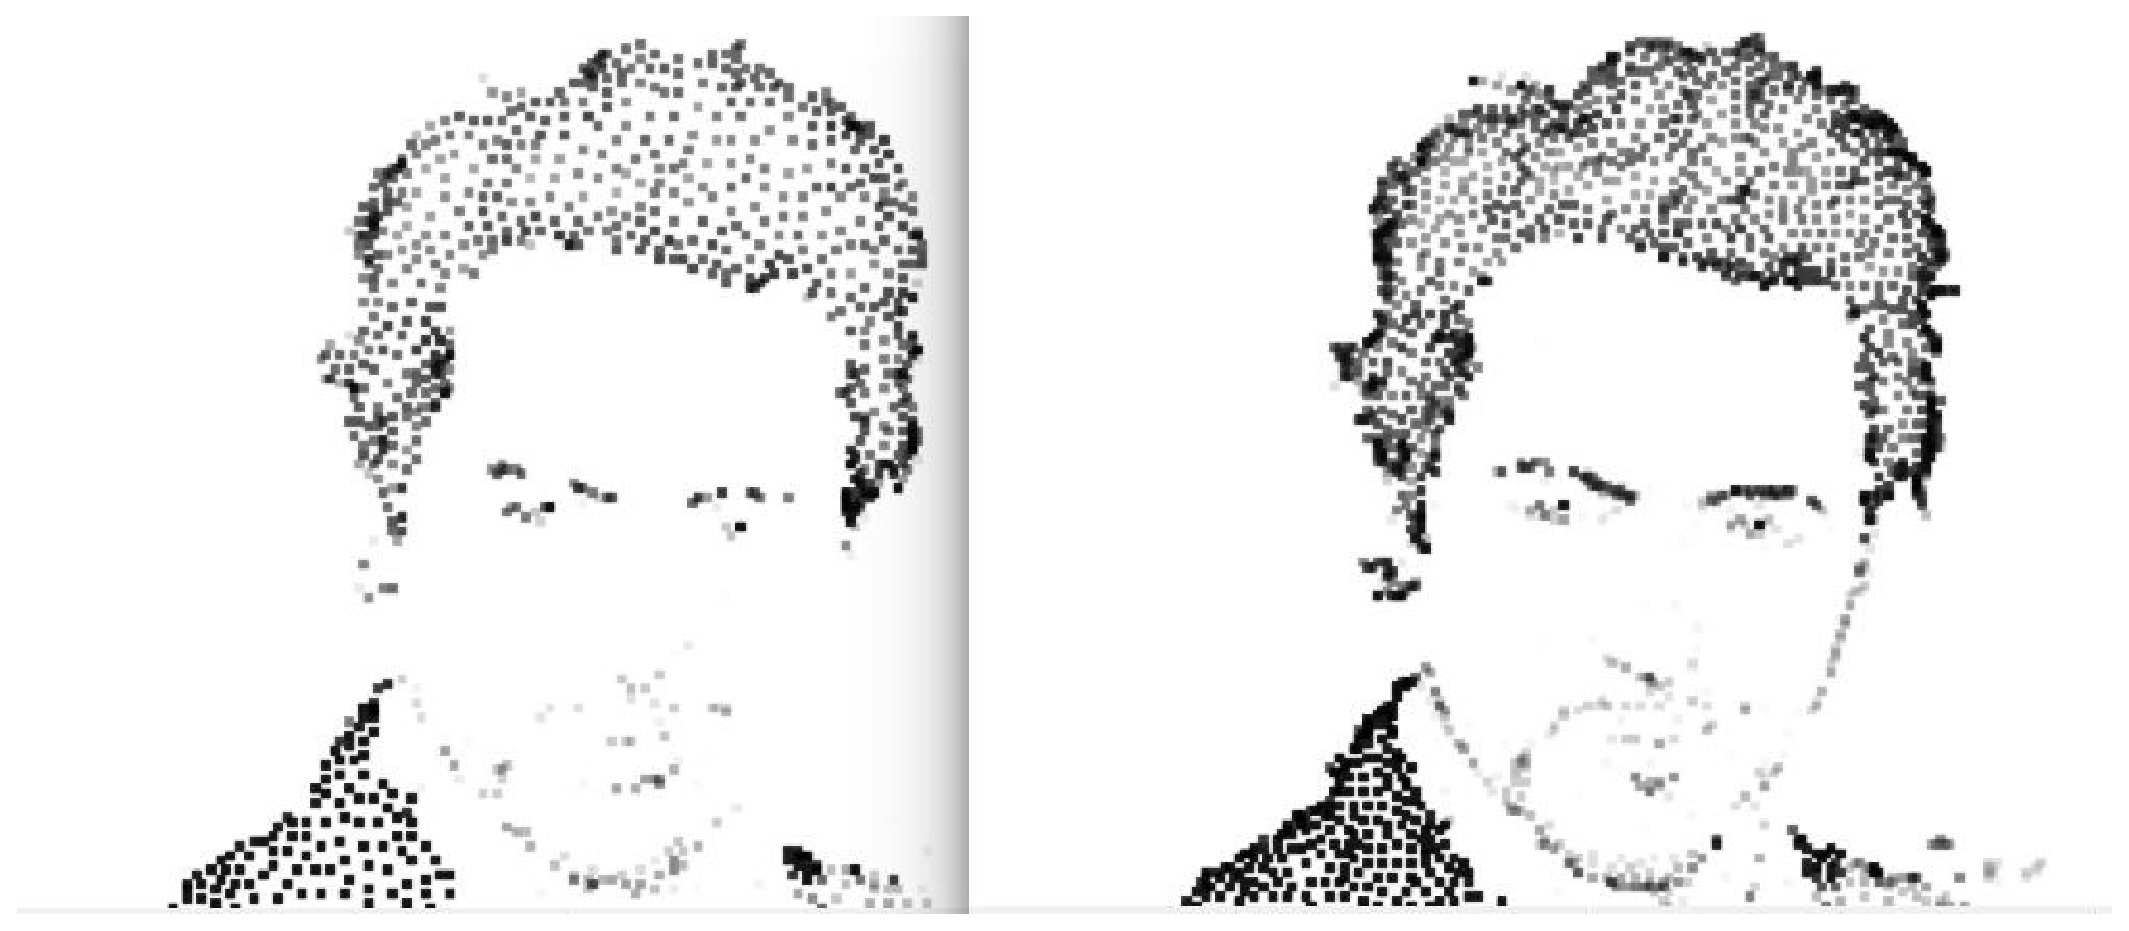
\includegraphics[width=0.80\textwidth]{figure2.eps}
\caption{Outputs from hedcuter}
\label{threadsVsSync}
\end{figure}
\begin{figure}[h!]
\centering
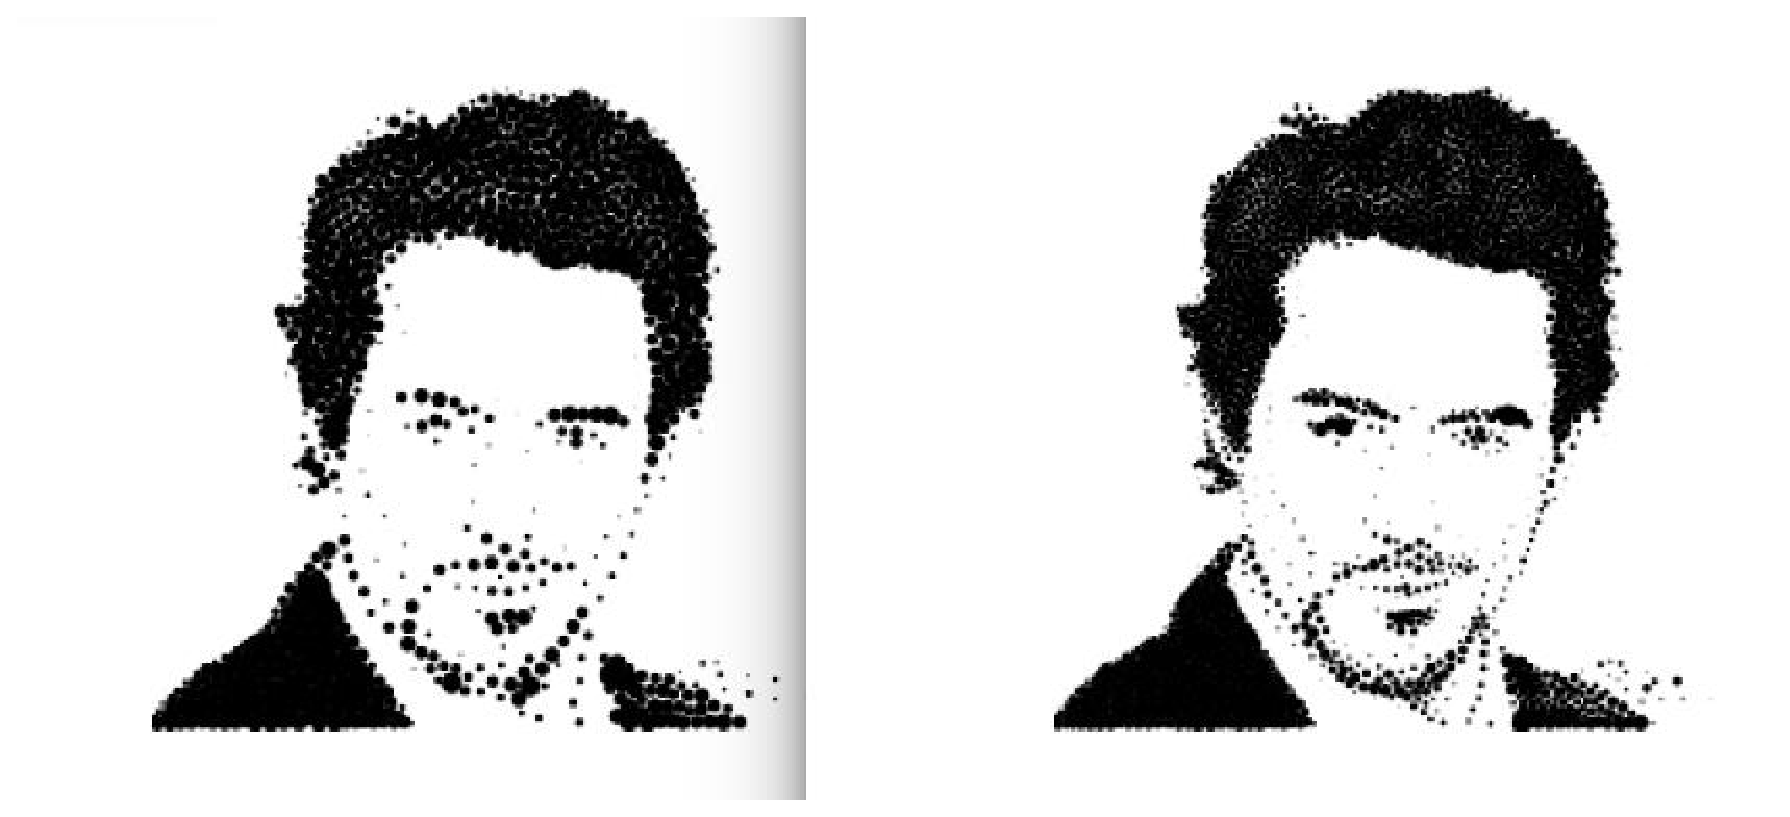
\includegraphics[width=0.80\textwidth]{figure3.eps}
\caption{Outputs from voronoi}
\label{threadsVsSync}
\end{figure}
\paragraph{2. The overall distribution will be the same for both methods. As Figure 2 and Figure 3 shows, the distribution remains the same. The difference here is that the one with more disks seems to be darker, because its density of disks is higher. And following these 2 methods, darker places deserve more disks. So the distribution should always be the same.}

\begin{figure}[h!]
\centering
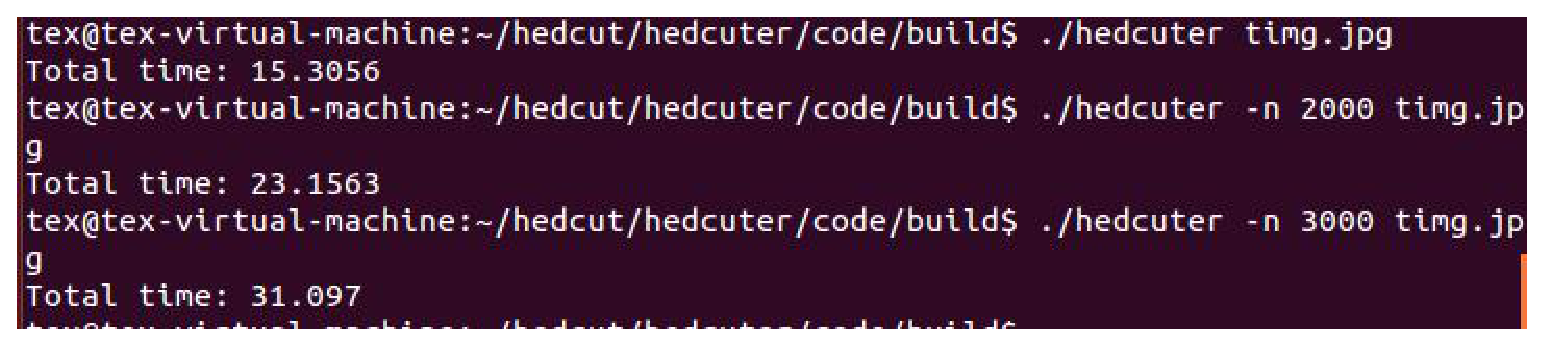
\includegraphics[width=0.80\textwidth]{figure4.eps}
\caption{Outputs from hedcuter}
\label{threadsVsSync}
\end{figure}
\begin{figure}[h!]
\centering
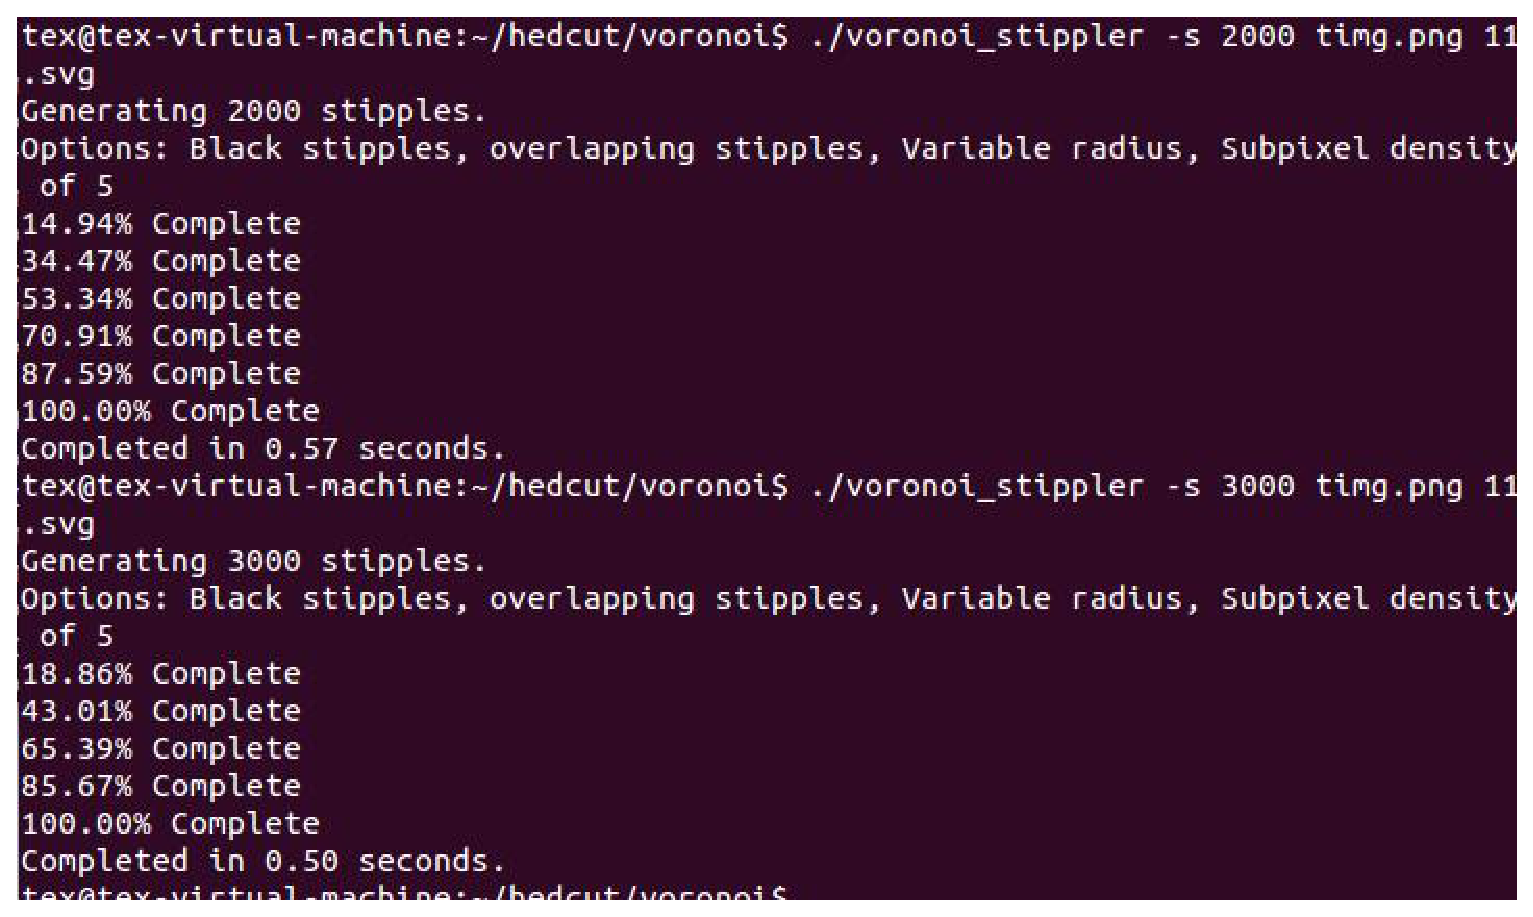
\includegraphics[width=0.80\textwidth]{figure5.eps}
\caption{Outputs from voronoi}
\label{threadsVsSync}
\end{figure}
\paragraph{3. As Figure 4 and 5 show, the voronoi method is always much faster than the other one when parameters are the same. And I think the reason hedcuter method is slower that much is because it generates the same virtual image repetitively. So, I take it as one of my improvement and the result is not bad. And other reasons are voronoi precomputes the sets of distribution and merge them at runtime. But hedcuter method is doing plane sweep from points with small x coordinates which is time consuming.}

\begin{figure}[h!]
\centering
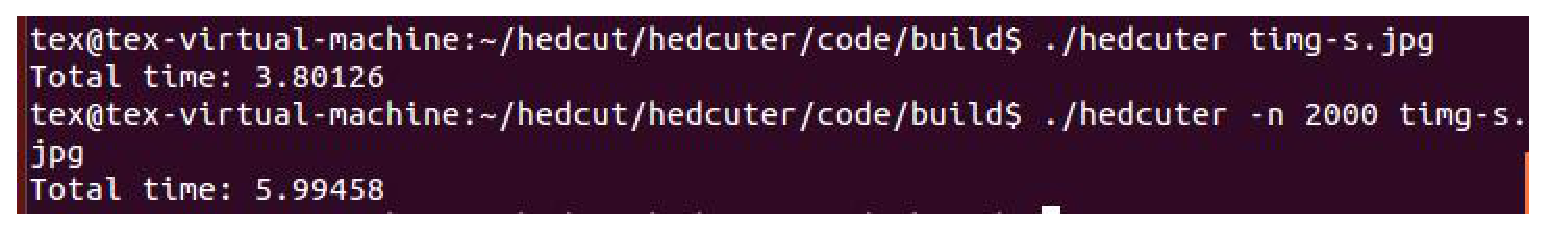
\includegraphics[width=0.80\textwidth]{figure6.eps}
\caption{Outputs from hedcuter}
\label{threadsVsSync}
\end{figure}
\begin{figure}[h!]
\centering
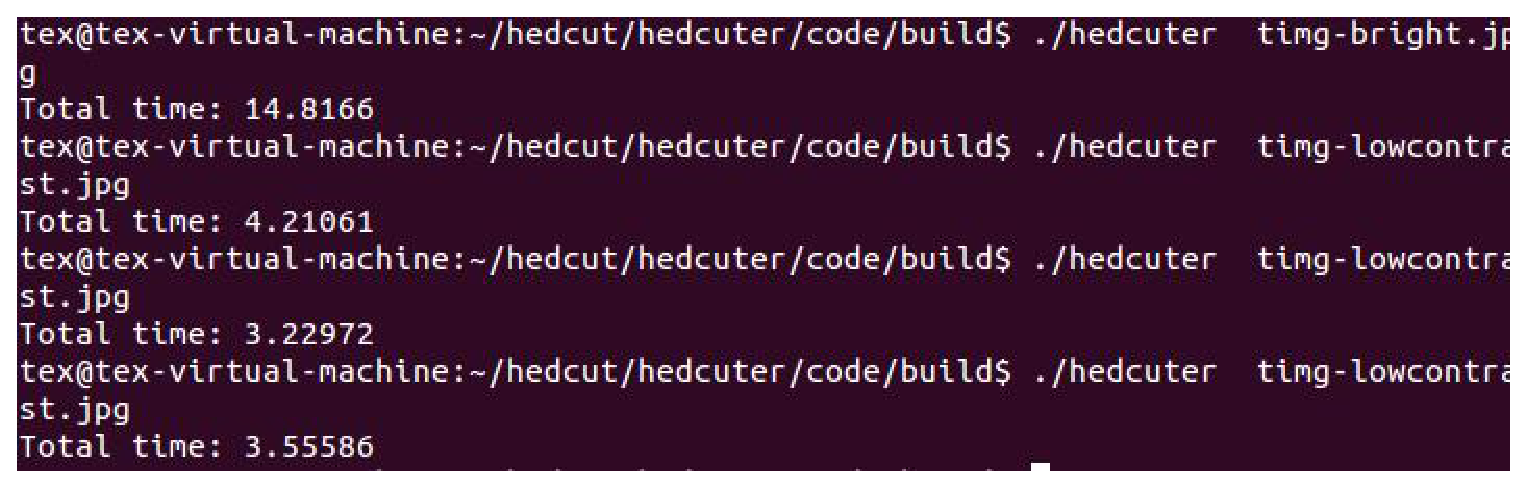
\includegraphics[width=0.80\textwidth]{figure7.eps}
\caption{Outputs from hedcuter}
\label{threadsVsSync}
\end{figure}
\begin{figure}[h!]
\centering
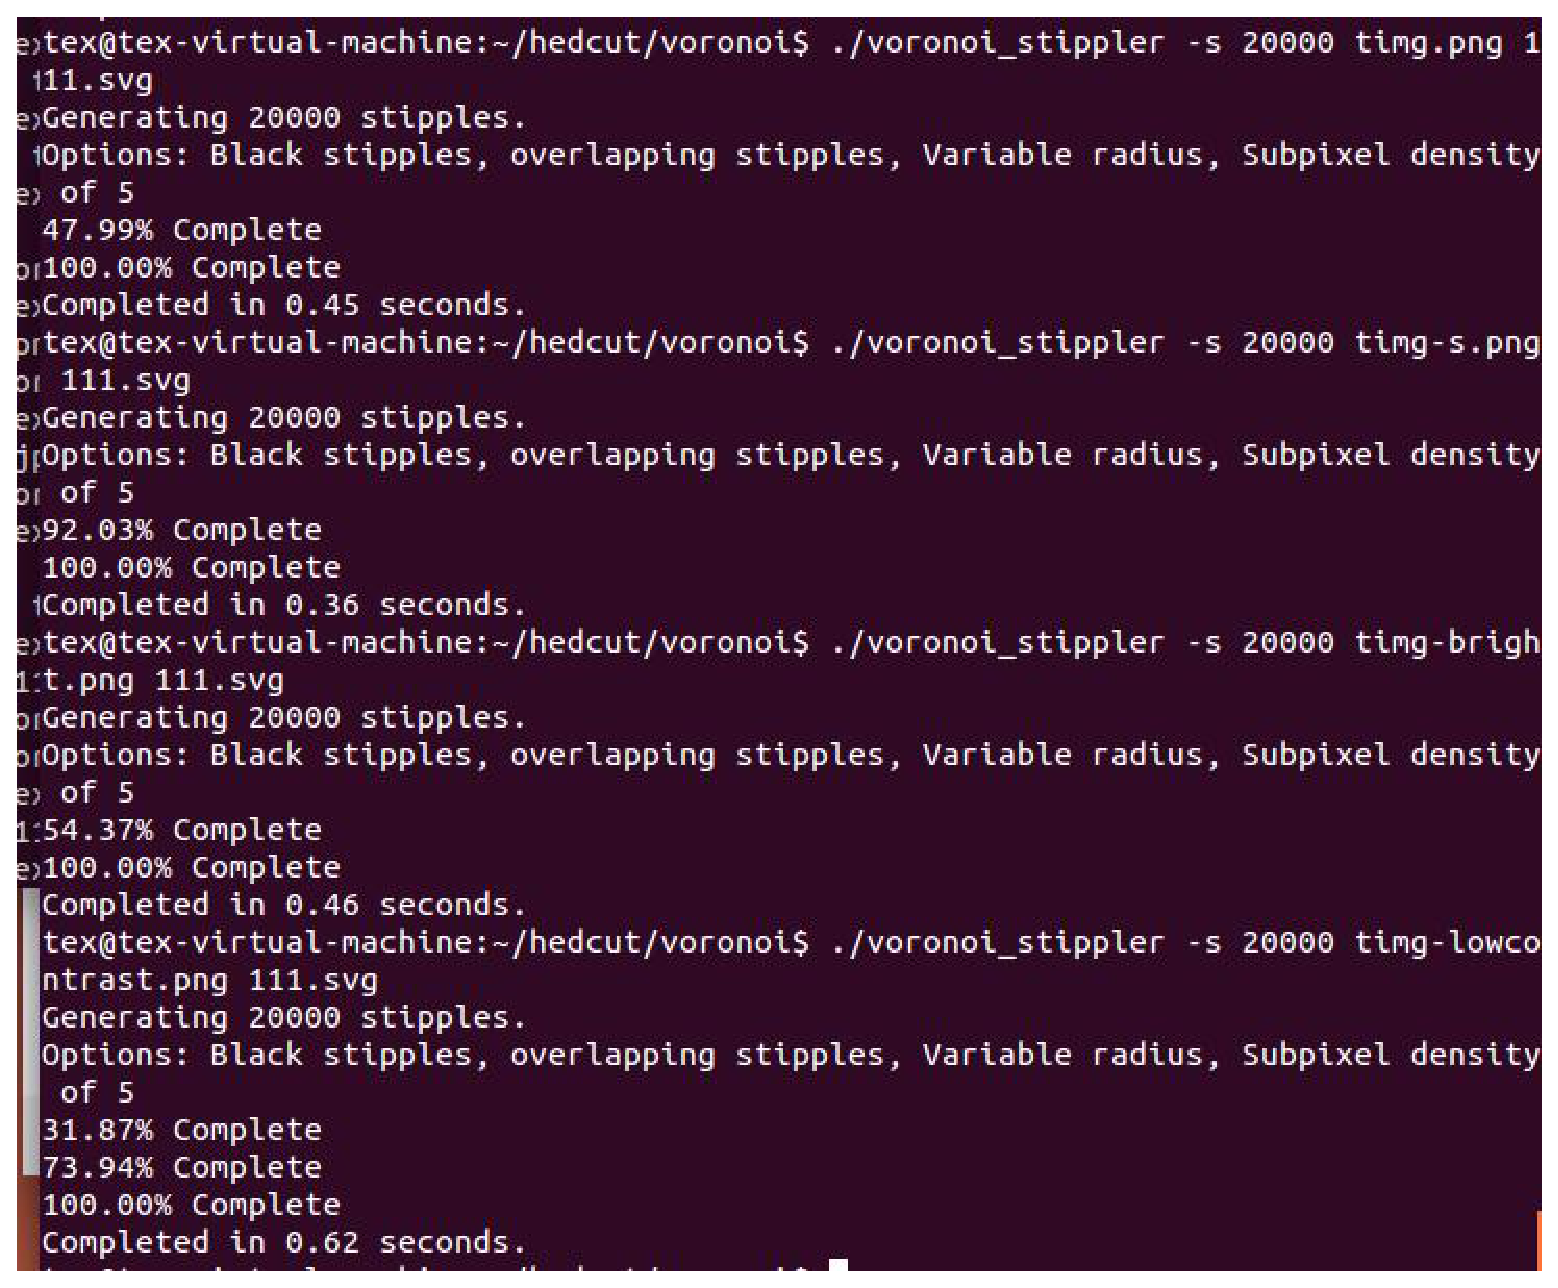
\includegraphics[width=0.80\textwidth]{figure8.eps}
\caption{Outputs from hedcuter}
\label{threadsVsSync}
\end{figure}
\paragraph{4. As figure 6, 7 and 8 show, for both methods, the same picture with smaller size consumes less time, because less pixels mean less iteration. For hedcuter method, it runs much faster with the low contrast picture. Because lowering contrast makes the picture darker. And when the picture is getting darker and darker, its distribution of disks becomes more uniform. Thus, the propagation task is achieved faster.  }

\begin{figure}[h!]
\centering
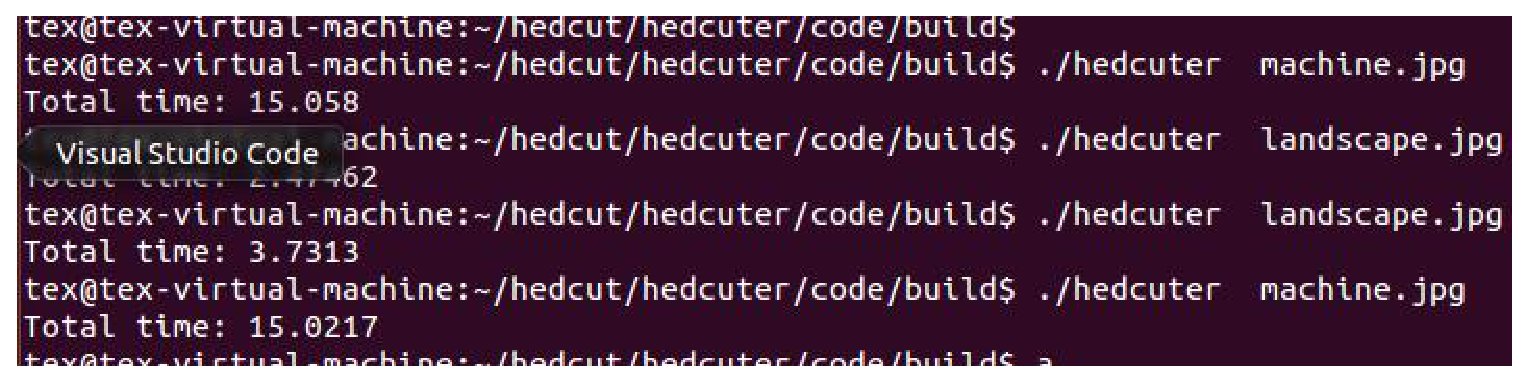
\includegraphics[width=0.80\textwidth]{figure9.eps}
\caption{Outputs from hedcuter}
\label{threadsVsSync}
\end{figure}
\begin{figure}[h!]
\centering
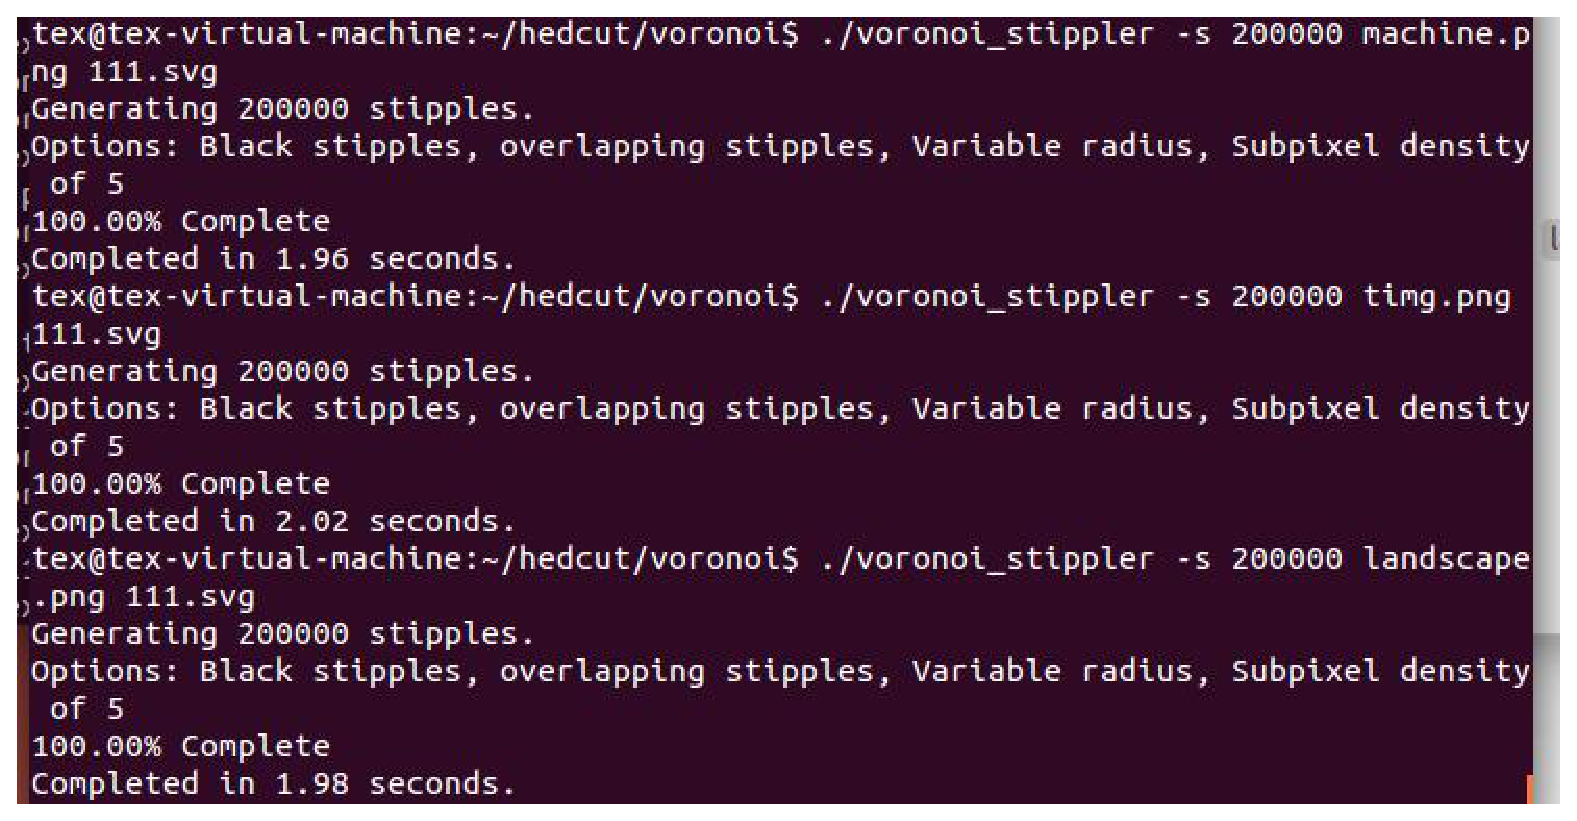
\includegraphics[width=0.80\textwidth]{figure10.eps}
\caption{Outputs from hedcuter}
\label{threadsVsSync}
\end{figure}
\paragraph{5. From Figure 9 and 10, different types of images have the approximate total time for voronoi method. But for hedcuter method, it performs better on landscape picture. I think it's because the landscape picture I chose is relatively darker than other types of pictures. So the reason is like for the pictures with low contrast value.  }

\begin{figure}[h!]
\centering
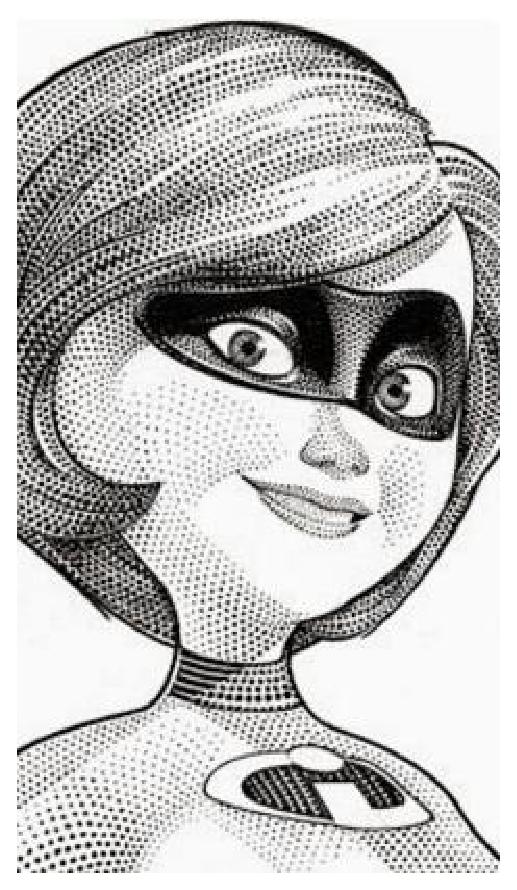
\includegraphics[width=3in]{figure11.eps}
\caption{hedcut image from Wall Street Journal}
\label{threadsVsSync}
\end{figure}
\begin{figure}[h!]
\centering
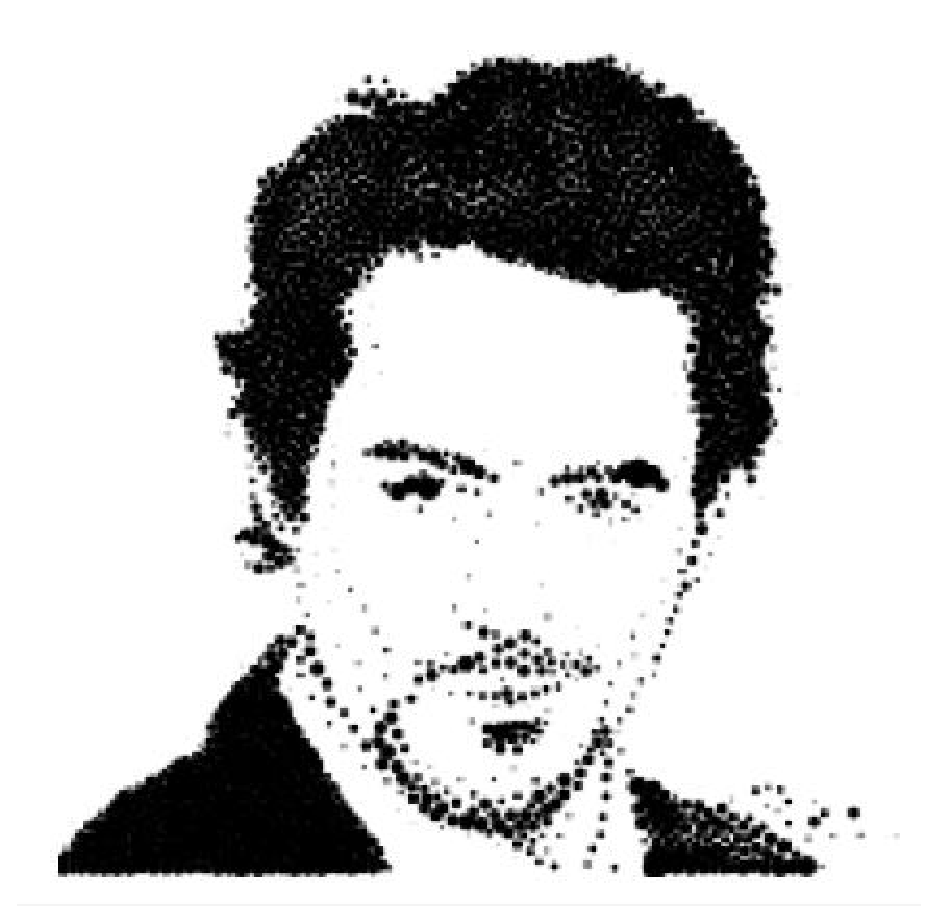
\includegraphics[width=0.80\textwidth]{figure12.eps}
\caption{Outputs from hedcuter}
\label{threadsVsSync}
\end{figure}
\paragraph{6. I think hedcut images from the Wall Street Journal are better than images generated by these 2 methods. As shown in Figure 11, it has smooth boundaries and more artistic distribution of disks. Figure 12 is generated by voronoi method from a 200x200 picture with 2000 disks. Although viewers are able to tell what's in the hedcut picture, its distribution of disks is not as natural as the one from Wall Street Journal.}
\section{Improvement of hedcuter method}
\begin{figure}[h!]
\centering
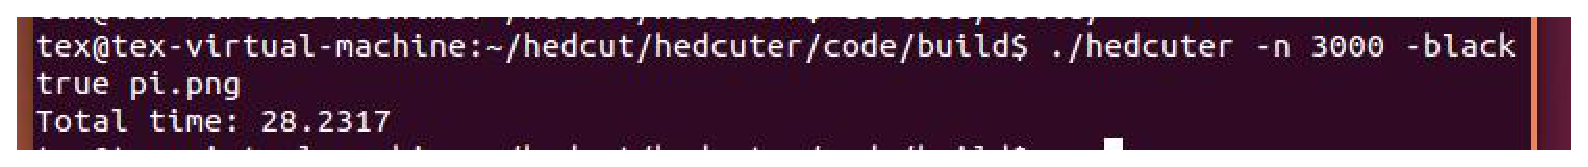
\includegraphics[width=0.80\textwidth]{figure13.eps}
\caption{output from original method}
\label{threadsVsSync}
\end{figure}
\begin{figure}[h!]
\centering
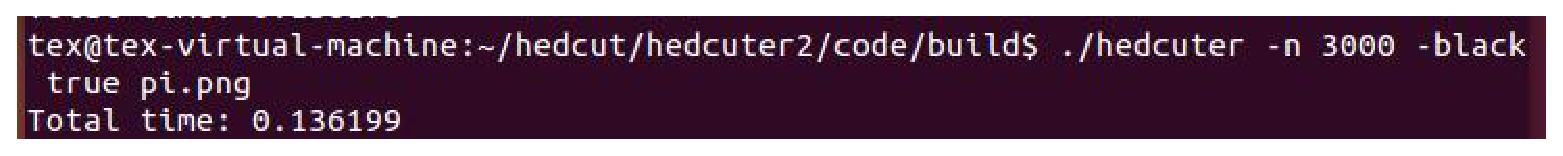
\includegraphics[width=0.80\textwidth]{figure14.eps}
\caption{outputs from new one}
\label{threadsVsSync}
\end{figure}
\paragraph{The first improvement is that I reorganized same codes so that the workload for vor and move\_sites methods are reduced. According to the original code, it seems like  each loop these two methods will generate a virtual high resolution image with the same parameters which means there is no need to do it repetitively. And it's also time consuming. Then, I changed that part of code so that the virtual image generating will be done only once. Figure 13 shows the total time the original program used to output the result. Figure 14 shows the total time the improved program used. The total time has reduced.}
\begin{figure}[h!]
\centering
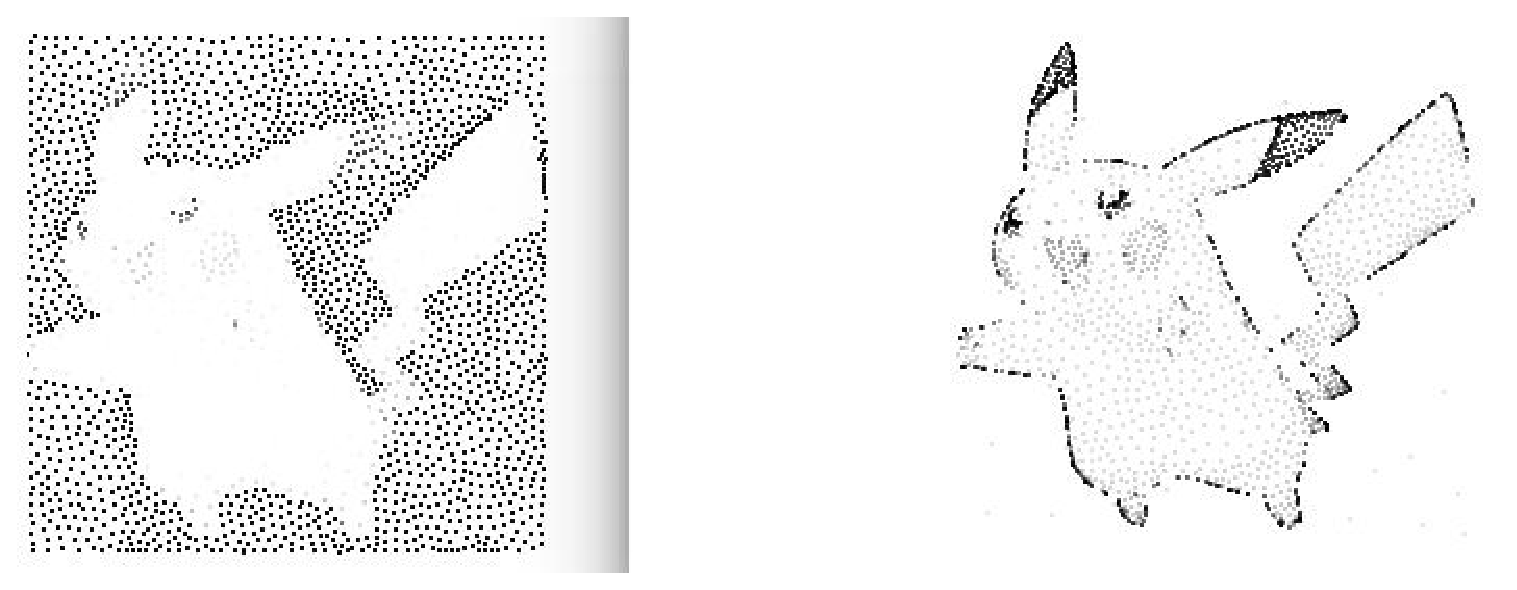
\includegraphics[width=0.80\textwidth]{figure15.eps}
\caption{comparison}
\label{threadsVsSync}
\end{figure}
\paragraph{The second improvement is that the program now can treat png files which contain transparent alpha channel correctly. The original version treats the transparent background as black which makes the output file weird. I modified main.cpp to make the input file lay on a white image. Fiqure 15 shows the comparison of the original program against the improved program with the same parameters. But when outputing colorful disks, the color of each disk is not always right. }
 \paragraph{Folder hedcuter2 has the codes for the first improvement. And folder hedcuter3 has the second improvement. And the output image makes more sense now.}
\bibliographystyle{plain}
\bibliography{report}

\end{document}


